\documentclass[11pt,a4paper]{article}

% ============================================================
% PACKAGES
% ============================================================
\usepackage[utf8]{inputenc}
\usepackage[T1]{fontenc}
\usepackage[margin=2.5cm]{geometry}
\usepackage[expansion=false]{microtype}
\usepackage{amsmath,amssymb,amsthm}
\usepackage{mathtools}
\usepackage{xcolor}
\usepackage{graphicx}
\usepackage{tikz}
\usepackage{pgfplots}
\usetikzlibrary{positioning,arrows.meta,shapes.geometric,fit,backgrounds,calc,decorations.pathreplacing,patterns,3d,shadings}
\pgfplotsset{compat=1.18}
\usepackage{booktabs}
\usepackage{array}
\usepackage{tabularx}
\usepackage{listings}
\usepackage{enumitem}
\usepackage{titling}
\usepackage{titlesec}
\usepackage{fancyhdr}
\usepackage{hyperref}
\usepackage{caption}
\usepackage{float}
\usepackage{quoting}

% ============================================================
% DESIGN TOKENS
% ============================================================
\definecolor{slate950}{HTML}{020617}
\definecolor{slate900}{HTML}{0f172a}
\definecolor{slate800}{HTML}{1e293b}
\definecolor{slate700}{HTML}{334155}
\definecolor{slate600}{HTML}{475569}
\definecolor{slate500}{HTML}{64748b}
\definecolor{slate400}{HTML}{94a3b8}
\definecolor{slate300}{HTML}{cbd5e1}
\definecolor{slate200}{HTML}{e2e8f0}
\definecolor{slate100}{HTML}{f1f5f9}
\definecolor{amber500}{HTML}{f59e0b}
\definecolor{amber400}{HTML}{fbbf24}
\definecolor{amber300}{HTML}{fcd34d}
\definecolor{emerald500}{HTML}{10b981}
\definecolor{emerald400}{HTML}{34d399}
\definecolor{rose500}{HTML}{f43f5e}
\definecolor{rose400}{HTML}{fb7185}
\definecolor{sky500}{HTML}{0ea5e9}
\definecolor{violet500}{HTML}{a855f7}

% ============================================================
% TYPOGRAPHY & STYLE
% ============================================================
\hypersetup{
  colorlinks=true,
  linkcolor=amber500,
  citecolor=amber500,
  urlcolor=sky500,
  pdftitle={TUNA Scenario Selector — Methodology and Design Specification v2.0},
  pdfauthor={Peter Verster},
  pdfsubject={Strategic foresight under TUNA conditions},
}

\titleformat{\section}{\Large\bfseries\color{slate900}}{\thesection}{1em}{}
\titleformat{\subsection}{\large\bfseries\color{slate800}}{\thesubsection}{1em}{}
\titleformat{\subsubsection}{\normalsize\bfseries\color{slate700}}{\thesubsubsection}{1em}{}

\pagestyle{fancy}
\fancyhf{}
\fancyhead[L]{\textcolor{slate500}{\small TUNA Scenario Selector}}
\fancyhead[R]{\textcolor{slate500}{\small Methodology \& Design v2.0}}
\fancyfoot[C]{\textcolor{slate500}{\small\thepage}}
\renewcommand{\headrulewidth}{0.4pt}
\renewcommand{\footrulewidth}{0pt}
\renewcommand{\headrule}{\hbox to\headwidth{\color{slate200}\leaders\hrule height \headrulewidth\hfill}}

\renewcommand{\quotingfont}{\itshape\color{slate700}}

\tikzset{
  every node/.style={font=\small},
  factor/.style={
    rectangle, rounded corners=2pt,
    draw=slate600, fill=slate100,
    minimum width=2.4cm, minimum height=0.7cm,
    align=center
  },
  highlight/.style={
    rectangle, rounded corners=2pt,
    draw=amber500, fill=amber500!15, very thick,
    minimum width=2.4cm, minimum height=0.7cm,
    align=center
  },
  arrow/.style={
    -{Stealth[length=3mm,width=2mm]},
    thick, draw=slate600
  },
  layer/.style={
    rectangle, rounded corners=4pt,
    minimum width=12cm, minimum height=1.4cm,
    align=center, font=\small
  },
}

% ============================================================
% TITLE PAGE
% ============================================================
\title{
  \vspace{-1.5cm}
  {\Huge\bfseries\color{slate900} TUNA Scenario Selector}\\[0.5em]
  {\Large\color{slate600} A morphological methodology for strategic seed generation}\\[0.3em]
  {\large\color{slate500} under turbulent, unpredictable, novel, and ambiguous conditions}\\[1em]
  {\normalsize\color{amber500}\bfseries Specification v2.0}
}
\author{
  {\large Peter Verster}\\
}
\date{\today}

\begin{document}

\maketitle
\thispagestyle{empty}

\vspace{0.8cm}

\begin{center}
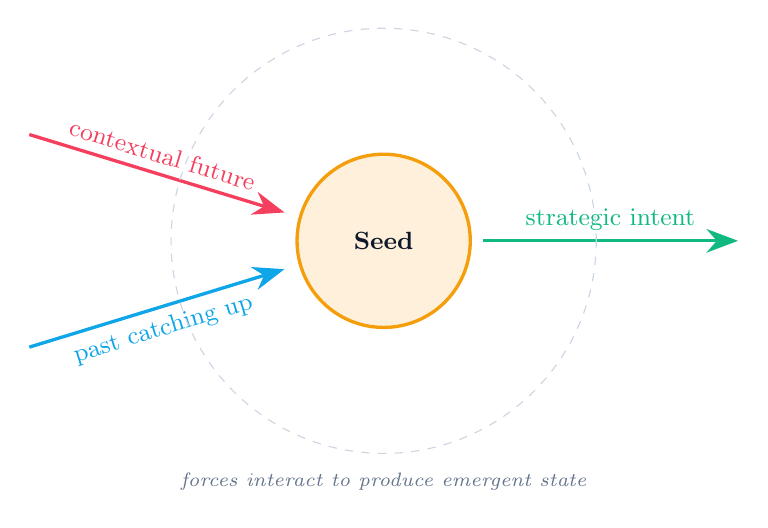
\begin{tikzpicture}[scale=0.9]
  \node[circle, draw=amber500, fill=amber500!15, very thick, minimum size=2.2cm] (m) at (0,0) {\textbf{\color{slate900}Seed}};
  \draw[-{Stealth[length=4mm,width=3mm]}, very thick, rose500] (-5,1.5) -- (-1.4,0.4) node[midway, above, sloped, color=rose500] {\small contextual future};
  \draw[-{Stealth[length=4mm,width=3mm]}, very thick, sky500] (-5,-1.5) -- (-1.4,-0.4) node[midway, below, sloped, color=sky500] {\small past catching up};
  \draw[-{Stealth[length=4mm,width=3mm]}, very thick, emerald500] (1.4,0) -- (5,0) node[midway, above, color=emerald500] {\small strategic intent};
  \draw[draw=slate300, dashed] (0,0) circle (3cm);
  \node[font=\scriptsize\itshape, color=slate500] at (0,-3.4) {forces interact to produce emergent state};
\end{tikzpicture}
\end{center}

\vspace{0.5cm}

\begin{quoting}
\noindent\textbf{Abstract.} This document specifies the methodology, mathematical foundation, algorithmic pipeline, and software architecture of the TUNA Scenario Selector — a tool that generates structured scenario seeds for strategic planning under deep uncertainty. The methodology integrates the Analytic Hierarchy Process for factor weighting, morphological analysis for combinatorial scenario space exploration, signed cross-consistency assessment with hard vetoes for coherence enforcement, arrows-of-time analysis with non-linear arrival estimation for temporal grounding, and a hybrid greedy-plus-local-search algorithm for diverse seed selection. The output is a small set of mathematically distinct, internally coherent, temporally anchored scenario seeds suitable as starting positions for narrative scenario development. Optional AI generation produces structured markdown narratives grounded in user-provided strategic context. Version 2.0 adds three principled improvements over v1.0: hard-veto filtering to defeat the compensation effect of pure aggregate-coupling, hill-climbing refinement to escape the myopia of greedy farthest-first traversal, and a saturating sigmoid arrival model that respects complexity-economics non-linearity.
\end{quoting}

\vfill
\hrule
\vspace{0.5em}
\noindent{\small\color{slate500} Document version 2.0 \textbullet{} Updated for hard vetoes, local-search refinement, non-linear arrival, AI generation pipeline, and deployment specifications}
\newpage

\tableofcontents
\newpage

% ============================================================
% PART I — PURPOSE
% ============================================================
\section{Purpose}

Strategic scenario planning is the standard practice for thinking about long-horizon futures under deep uncertainty. The dominant method, sometimes called the GBN or intuitive logics approach after the Global Business Network where it was codified by Schwartz, Wack, and Ogilvy in the 1980s, has been the consensus practice in corporate strategy for forty years. It produces four scenarios by selecting two high-impact, high-uncertainty driving forces as axes of a 2$\times$2 matrix. The method works in the sense that it produces scenarios strategists and boards can engage with, but it has three structural weaknesses that experienced practitioners work around informally.

\subsection{Structural weaknesses of the 2$\times$2 method}

\begin{enumerate}[leftmargin=*]
  \item \textbf{No enforced independence.} Two driving forces can both score highly on impact and uncertainty but be causally entangled, so the four quadrants of the matrix collapse into two effective futures or one. Energy security and geopolitical stability, for instance, both look like good axes — but in practice energy security is largely driven by geopolitical stability, so the ``low geopolitics, high energy security'' quadrant doesn't represent a coherent world.
  \item \textbf{Static treatment of time.} The 2$\times$2 method produces scenarios as spatial configurations rather than transitional moments. In TUNA conditions, where the environment is, in W.\ Brian Arthur's framing, a complex adaptive system that bifurcates rather than evolves smoothly, the moments of structural transition are precisely what scenario planning should illuminate, and the 2$\times$2 method is poorly suited to capturing them.
  \item \textbf{Opaque reasoning chain.} When a stakeholder asks ``why these four scenarios rather than four others'', the answer is ``this was our judgement''. Increasingly insufficient for sophisticated audiences that expect reasoning transparency, and meaningless for any kind of audit or stress test.
\end{enumerate}

\subsection{What this tool addresses}

The tool addresses all three weaknesses through a structured pipeline that combines AHP for factor weighting, morphological analysis for scenario space exploration, signed coupling with hard vetoes for coherence enforcement, arrows-of-time analysis for temporal grounding, and a refined diverse-seed selection algorithm. The output is a small set of scenario seeds — typically four — that are mathematically distinct, internally coherent, anchored in time, and defended by an auditable chain of judgement.

\textbf{These seeds are not finished scenarios.} They are starting positions for narrative scenario development. Optional AI generation produces a structured markdown narrative for each seed, but the strategist still owns the final story, signals, and strategic implications. The tool's contribution is to ensure narrative work begins from a defensible structural position rather than from intuition alone.

% ============================================================
% PART II — METHODOLOGICAL FOUNDATION
% ============================================================
\section{Methodological foundation}

The solution integrates four distinct methodological traditions. Each is summarised here at the level of detail required to apply it correctly.

\subsection{Causal Texture Theory and Knightian Uncertainty}

Fred Emery and Eric Trist (1965) classified organisational environments into four types based on causal interconnection: Placid-Randomised, Placid-Clustered, Disturbed-Reactive, and Turbulent Fields. The fourth — turbulent fields — is the environment for which the present tool is designed: dynamic, highly interconnected, with changes amplifying through the system in unpredictable ways. Frank Knight (1921) distinguished \emph{risk} (probabilities knowable, calculable, insurable) from \emph{uncertainty} (probabilities unknowable, situation novel, irreducible to mathematics). The intersection of turbulent-field dynamics with Knightian uncertainty is what Oxford's Saïd Business School calls TUNA conditions: \textbf{Turbulent}, \textbf{Unpredictable}, \textbf{Novel}, \textbf{Ambiguous}. Scenarios are not probabilistic forecasts; they are imaginative explorations of plausible futures under irreducible uncertainty.

\begin{figure}[H]
\centering
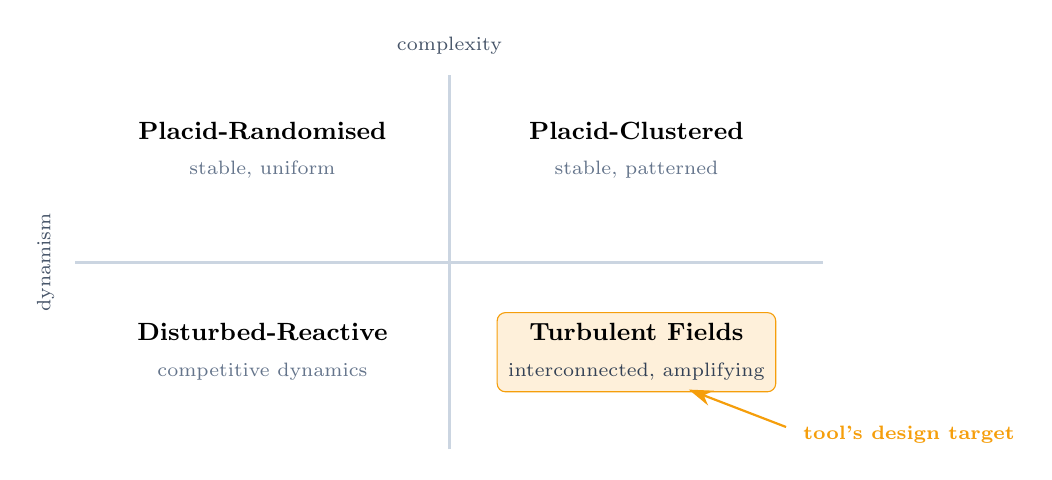
\begin{tikzpicture}[scale=0.95]
  \draw[slate300, thick] (0,0) -- (10,0);
  \draw[slate300, thick] (5,-2.5) -- (5,2.5);
  \node[align=center] at (2.5,1.5) {\small\textbf{Placid-Randomised}\\[2pt] \scriptsize\color{slate500}stable, uniform};
  \node[align=center] at (7.5,1.5) {\small\textbf{Placid-Clustered}\\[2pt] \scriptsize\color{slate500}stable, patterned};
  \node[align=center] at (2.5,-1.2) {\small\textbf{Disturbed-Reactive}\\[2pt] \scriptsize\color{slate500}competitive dynamics};
  \node[align=center, fill=amber500!15, draw=amber500, rounded corners=3pt, inner sep=4pt] at (7.5,-1.2) {\small\textbf{Turbulent Fields}\\[2pt] \scriptsize\color{slate700}interconnected, amplifying};
  \node[color=slate600, font=\scriptsize] at (5,2.9) {complexity};
  \node[color=slate600, font=\scriptsize, rotate=90] at (-0.4,0) {dynamism};
  \draw[-{Stealth[length=3mm,width=2mm]}, amber500, thick] (9.5,-2.2) -- (8.2,-1.7);
  \node[color=amber500, font=\scriptsize\bfseries, anchor=west] at (9.6,-2.3) {tool's design target};
\end{tikzpicture}
\caption{Emery and Trist's four environmental types. The TUNA Scenario Selector is designed for turbulent fields where complexity and dynamism reinforce each other.}
\end{figure}

\subsection{W. Brian Arthur's complexity economics}

Arthur's work on combinatorial technology evolution and increasing returns provides the structural model for \emph{why} TUNA conditions exist. Three Arthurian claims underpin the methodology:

\begin{itemize}[leftmargin=*]
  \item \textbf{Combinatorial evolution.} Technologies recombine at exponential rates. Each new combination opens further combinations, producing the densely interconnected web of innovation that turbulent fields are made of.
  \item \textbf{Increasing returns.} Positive feedback loops drive runaway dynamics rather than equilibrium. Network effects, lock-in, learning curves, and standard adoption all amplify the dominant trajectory rather than damping it.
  \item \textbf{Bifurcation.} Systems accumulate tension until the interaction of forces produces qualitatively new configurations that neither force alone would have generated. The strategist's task is not to predict which bifurcation will happen but to imagine plausible \emph{post-bifurcation realities} and prepare for them.
\end{itemize}

\subsection{Analytic Hierarchy Process}

Saaty (1977) decomposes a complex decision into a hierarchy of criteria and alternatives, then derives priorities through pairwise comparisons on a 1--9 ratio scale. The principal eigenvector of the resulting comparison matrix yields the priority vector; the consistency ratio measures internal contradiction in the strategist's judgements. The tool uses AHP for the first half of the workflow: weighting evaluation criteria and scoring factors against each criterion, producing a defensible global priority for each candidate factor.

\subsection{Morphological Analysis with Hard-Veto Augmentation}

Zwicky (1969) and Ritchey (2011) treat each factor as a dimension with a small set of discrete states and exhaustively enumerate configurations. For $N$ factors with $K$ states each, the morphological space contains $K^N$ configurations. Cross-Consistency Assessment (CCA) filters this space by removing internally contradictory configurations.

The tool implements a \textbf{two-layer filter} that combines the rigour of CCA with the practicality of aggregate coupling. The first layer is a set of \emph{hard vetoes} — explicit factor-state pairs the strategist marks as logically impossible. Any seed containing a vetoed pair is removed unconditionally before scoring. The second layer is the soft \emph{aggregate-coupling coherence score} — a continuous penalty function that captures graded incompatibility between states under signed coupling. The two layers together capture both the absolute and the gradient kinds of structural inconsistency, addressing the compensation effect that pure aggregate-coupling allows.

\subsection{The three arrows of time}

The Oxford Scenario Planning Approach distinguishes three temporal arrows. They are best understood as \emph{forces in continuous play}, not events that meet at a moment. Each arrow names a different origin from which influence reaches the present: the contextual future flows backward as anticipated regulation, demographic change, or technological maturity already implicit in today's research; the past pushes forward as accumulated lock-in, sunk infrastructure, and demographic momentum; strategic intent projects outward from present choices toward an imagined target.

Bifurcation does not occur when these arrows ``arrive at the same time''. They are always all in play simultaneously. Bifurcation occurs when forces arising from different temporal origins \emph{interact} to produce emergent states that neither force alone implies. Future-borne regulation plus past-borne underinvestment can together produce a third state — say, a stranded-asset crisis — that neither the regulatory trajectory nor the investment trajectory contained as a possibility on its own. The methodology's interest in factor coupling is precisely this: identifying the configurations where forces from different origins interact in ways that generate qualitatively new outcomes.

\begin{figure}[H]
\centering
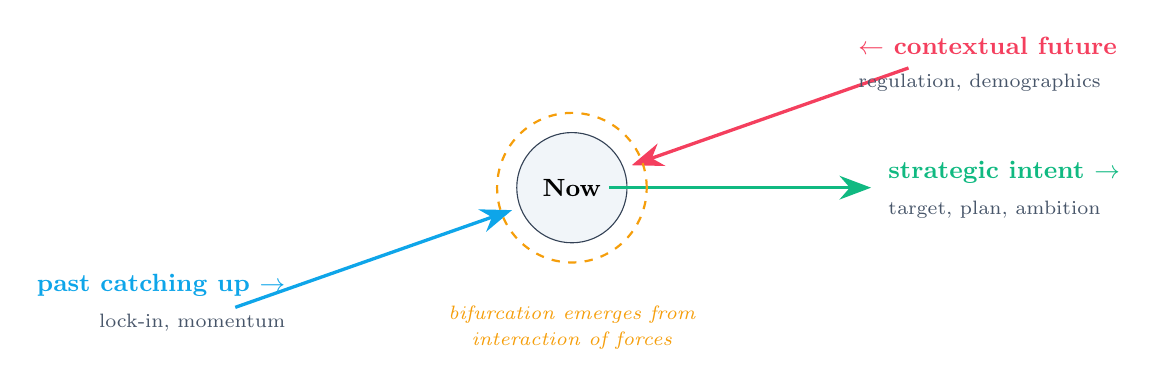
\begin{tikzpicture}[scale=0.95]
  \node[circle, draw=slate700, fill=slate100, minimum size=1.4cm] (obs) at (5,0) {\small\textbf{Now}};
  \draw[-{Stealth[length=4mm,width=3mm]}, very thick, rose500] (9.5,1.6) -- (5.8,0.3);
  \node[color=rose500, font=\small\bfseries, anchor=west] at (8.7,1.9) {$\leftarrow$ contextual future};
  \node[color=slate600, font=\scriptsize, anchor=west] at (8.7,1.4) {regulation, demographics};
  \draw[-{Stealth[length=4mm,width=3mm]}, very thick, emerald500] (5.5,0) -- (9.0,0);
  \node[color=emerald500, font=\small\bfseries, anchor=west] at (9.1,0.2) {strategic intent $\rightarrow$};
  \node[color=slate600, font=\scriptsize, anchor=west] at (9.1,-0.3) {target, plan, ambition};
  \draw[-{Stealth[length=4mm,width=3mm]}, very thick, sky500] (0.5,-1.6) -- (4.2,-0.3);
  \node[color=sky500, font=\small\bfseries, anchor=east] at (1.3,-1.3) {past catching up $\rightarrow$};
  \node[color=slate600, font=\scriptsize, anchor=east] at (1.3,-1.8) {lock-in, momentum};
  \draw[draw=amber500, dashed, thick] (5,0) circle (1.0cm);
  \node[color=amber500, font=\scriptsize\itshape] at (5,-1.7) {bifurcation emerges from};
  \node[color=amber500, font=\scriptsize\itshape] at (5,-2.05) {interaction of forces};
\end{tikzpicture}
\caption{The three arrows of time from the Oxford Scenario Planning Approach. They are sources of force, always in play, not events that arrive at a moment. The tool encodes the red arrow's properties (velocity, proximity to threshold) and the blue arrow's properties (path-dependency, accumulated lock-in) as factor-level inputs, and uses the coupling matrix to capture how forces from different origins interact. Emergent third states — bifurcations — appear in the morphological space as configurations where coupled high-criticality factors take extreme values simultaneously, indicating a region where force interaction is structurally dense. The green arrow is downstream — the strategy that gets tested against the seed set.}
\end{figure}

% ============================================================
% PART III — VECTOR-SPACE MENTAL MODEL
% ============================================================
\section{The vector-space mental model}

Geometrically, the methodology has a clean interpretation that makes it easier to explain and reason about. Every scenario is a point in a high-dimensional space. Each factor is one of the dimensions, and each scenario's coordinate on that dimension is determined by the state the factor takes.

\subsection{The morphological space as a discrete lattice}

With $N$ factors and $K$ possible states each, the morphological space is the set of all vectors $S \in \{v_0, v_1, \ldots, v_{K-1}\}^N$ — the complete discrete lattice of $K^N$ points in $N$-dimensional space. Each point is one possible scenario.

\begin{figure}[H]
\centering
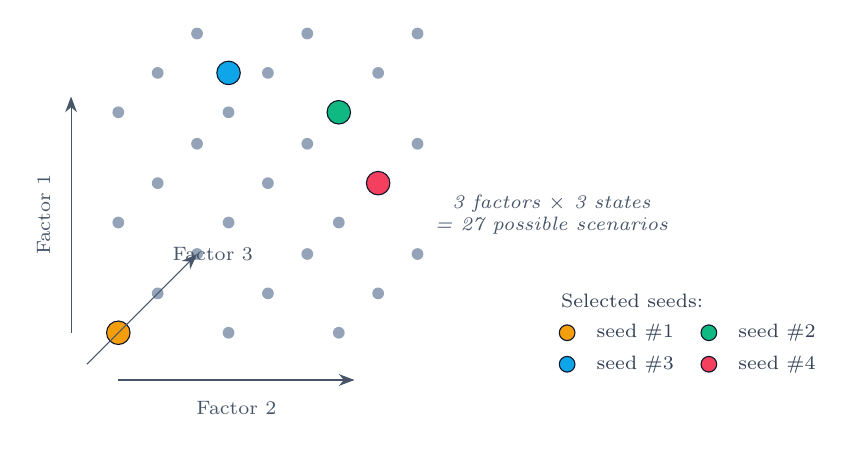
\begin{tikzpicture}[scale=1.0]
  \foreach \x in {0,1,2}
    \foreach \y in {0,1,2}
      \foreach \z in {0,1,2} {
        \pgfmathsetmacro{\px}{\x*1.4 + \z*0.5}
        \pgfmathsetmacro{\py}{\y*1.4 + \z*0.5}
        \node[circle, fill=slate400, inner sep=1.5pt] at (\px,\py) {};
      }
  \node[circle, fill=amber500, inner sep=3pt, draw=slate900] at (0,0) {};
  \node[circle, fill=emerald500, inner sep=3pt, draw=slate900] at (2.8,2.8) {};
  \node[circle, fill=sky500, inner sep=3pt, draw=slate900] at (1.4,2.8+0.5) {};
  \node[circle, fill=rose500, inner sep=3pt, draw=slate900] at (2.8+0.5,1.4+0.5) {};
  \draw[-{Stealth[length=2mm,width=1.5mm]}, slate600] (-0.6,0) -- (-0.6,3);
  \node[color=slate600, font=\scriptsize, rotate=90] at (-0.95,1.5) {Factor 1};
  \draw[-{Stealth[length=2mm,width=1.5mm]}, slate600] (0,-0.6) -- (3,-0.6);
  \node[color=slate600, font=\scriptsize] at (1.5,-0.95) {Factor 2};
  \draw[-{Stealth[length=2mm,width=1.5mm]}, slate600] (-0.4,-0.4) -- (1.0,1.0);
  \node[color=slate600, font=\scriptsize] at (1.2,1.0) {Factor 3};
  \node[font=\scriptsize\itshape, color=slate600, align=center] at (5.5,1.5) {3 factors $\times$ 3 states\\ = 27 possible scenarios};
  \node[font=\scriptsize, color=slate700, anchor=west] at (5.5,0.4) {Selected seeds:};
  \node[circle, fill=amber500, inner sep=2pt, draw=slate900] at (5.7,0) {};
  \node[font=\scriptsize, color=slate700, anchor=west] at (5.95,0) {seed \#1};
  \node[circle, fill=emerald500, inner sep=2pt, draw=slate900] at (7.5,0) {};
  \node[font=\scriptsize, color=slate700, anchor=west] at (7.75,0) {seed \#2};
  \node[circle, fill=sky500, inner sep=2pt, draw=slate900] at (5.7,-0.4) {};
  \node[font=\scriptsize, color=slate700, anchor=west] at (5.95,-0.4) {seed \#3};
  \node[circle, fill=rose500, inner sep=2pt, draw=slate900] at (7.5,-0.4) {};
  \node[font=\scriptsize, color=slate700, anchor=west] at (7.75,-0.4) {seed \#4};
\end{tikzpicture}
\caption{The morphological space visualised as a discrete lattice for the trivial $N=3$, $K=3$ case. Every grey point is one possible scenario; coloured points are the four selected seeds. Real scenario problems use 6--8 factors, producing 729 to 6{,}561 lattice points — too many to enumerate by hand, trivial for a computer.}
\end{figure}

\subsection{The relationship to embeddings}

Practitioners familiar with embeddings will recognise the structure: points in high-dimensional space where directions and distances carry meaning. Two important refinements distinguish this morphological space from typical machine-learning embeddings:

\begin{enumerate}[leftmargin=*]
  \item \textbf{Embeddings are usually continuous; the morphological space is discrete.} A typical embedding lives in continuous $\mathbb{R}^n$ where every real-numbered point is valid. The morphological space is a finite lattice — only $K^N$ specific points exist, the ones whose coordinates are drawn from the allowed state values. The space is $N$-dimensional but it is a sparse grid, not a continuous volume.
  \item \textbf{Weights don't change the lengths of vectors — they change the metric.} The seed $[+1, -1, 0, +1, -1, 0]$ has the same coordinates whether or not AHP weighting has been applied. What the weights do is change how \emph{distance is measured} between vectors. A weighted Hamming distance treats a difference on a heavyweight axis as worth more than the same difference on a lightweight axis. The geometry of the space is unchanged; the ruler has been re-scaled.
\end{enumerate}

\begin{figure}[H]
\centering
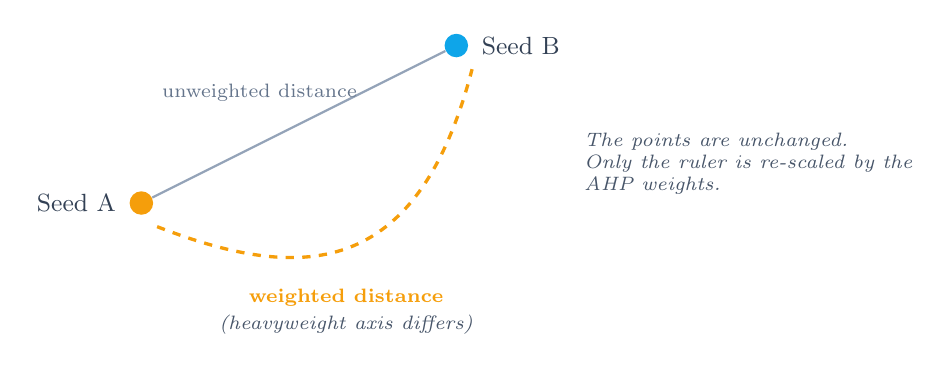
\begin{tikzpicture}[scale=1.0]
  \node[circle, fill=amber500, inner sep=3pt] (a) at (0,0) {};
  \node[circle, fill=sky500, inner sep=3pt] (b) at (4,2) {};
  \node[font=\small, color=slate700, anchor=east] at (-0.2,0) {Seed A};
  \node[font=\small, color=slate700, anchor=west] at (4.2,2) {Seed B};
  \draw[draw=slate400, thick] (a) -- (b);
  \node[font=\scriptsize, color=slate500] at (1.5,1.4) {unweighted distance};
  \draw[draw=amber500, very thick, dashed] (0.2,-0.3) .. controls (2,-1) and (3.5,-1) .. (4.2,1.7);
  \node[font=\scriptsize\bfseries, color=amber500] at (2.6,-1.2) {weighted distance};
  \node[font=\scriptsize\itshape, color=slate600] at (2.6,-1.55) {(heavyweight axis differs)};
  \node[font=\scriptsize\itshape, color=slate600, anchor=west, align=left] at (5.5,0.5) {The points are unchanged.\\Only the ruler is re-scaled by the\\ AHP weights.};
\end{tikzpicture}
\caption{AHP weighting transforms the metric, not the geometry. Two scenarios that are equally far apart by simple Hamming distance can be far apart \emph{or} close together once weights are applied, depending on which factors differ.}
\end{figure}

\subsection{What the algorithm does, geometrically}

The selection algorithm searches the lattice for points satisfying three properties simultaneously: \textbf{importance} (heavy in the dimensions with high AHP weight), \textbf{coherence} (internally consistent under coupling constraints and not in violation of any hard vetoes), and \textbf{convergence potential} (high-criticality dimensions at extreme states). It then picks four points that are mutually far apart under the weighted metric, with a hill-climbing refinement to escape locally suboptimal greedy commitments.

The methodology's deeper claim is not that it discovers exotic scenarios humans wouldn't have found. It is that it \emph{eliminates} the trivial, contradictory, vetoed, or near-duplicate configurations and surfaces the small set that genuinely deserves narrative work. It is a filter on combinatorial overwhelm, which is a more honest claim than ``it generates scenarios''.

\subsection{The size of the space}

The morphological space grows exponentially with the number of factors. Specifically, the count is $K^N$ for uniform state cardinality, or $\prod_i K_i$ for non-uniform.

\begin{figure}[H]
\centering
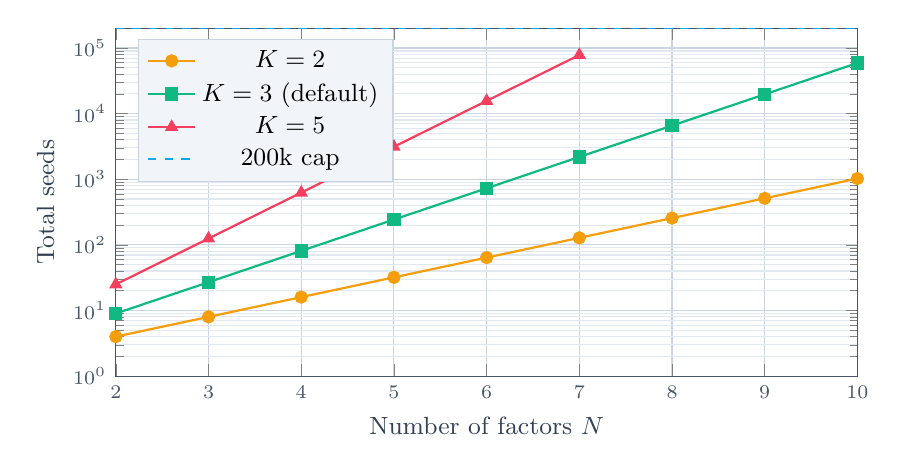
\begin{tikzpicture}
  \begin{semilogyaxis}[
    width=11cm, height=6cm,
    xlabel={Number of factors $N$},
    ylabel={Total seeds},
    xmin=2, xmax=10,
    ymin=1, ymax=200000,
    grid=both,
    grid style={slate200},
    major grid style={slate300},
    axis line style={slate600},
    tick label style={font=\scriptsize, color=slate600},
    label style={font=\small, color=slate700},
    legend style={font=\scriptsize, draw=slate300, fill=slate100},
    legend pos=north west,
  ]
    \addplot[mark=*, color=amber500, thick] coordinates {
      (2,4) (3,8) (4,16) (5,32) (6,64) (7,128) (8,256) (9,512) (10,1024)
    };
    \addlegendentry{$K=2$}
    \addplot[mark=square*, color=emerald500, thick] coordinates {
      (2,9) (3,27) (4,81) (5,243) (6,729) (7,2187) (8,6561) (9,19683) (10,59049)
    };
    \addlegendentry{$K=3$ (default)}
    \addplot[mark=triangle*, color=rose500, thick] coordinates {
      (2,25) (3,125) (4,625) (5,3125) (6,15625) (7,78125)
    };
    \addlegendentry{$K=5$}
    \addplot[domain=2:10, dashed, sky500, thick] {200000};
    \addlegendentry{200k cap}
  \end{semilogyaxis}
\end{tikzpicture}
\caption{Morphological space size on a logarithmic scale. The default configuration of eight factors and three states produces 6{,}561 candidate seeds — comfortable for brute-force enumeration. The tool caps at 200{,}000 seeds; beyond that, heuristic search replaces brute force.}
\end{figure}

% ============================================================
% PART IV — THE PIPELINE
% ============================================================
\section{The pipeline}

The tool implements a ten-step workflow taking raw judgement about factors and criteria as input, producing a small set of named scenario seeds with optional AI-generated narratives as output.

\begin{figure}[H]
\centering
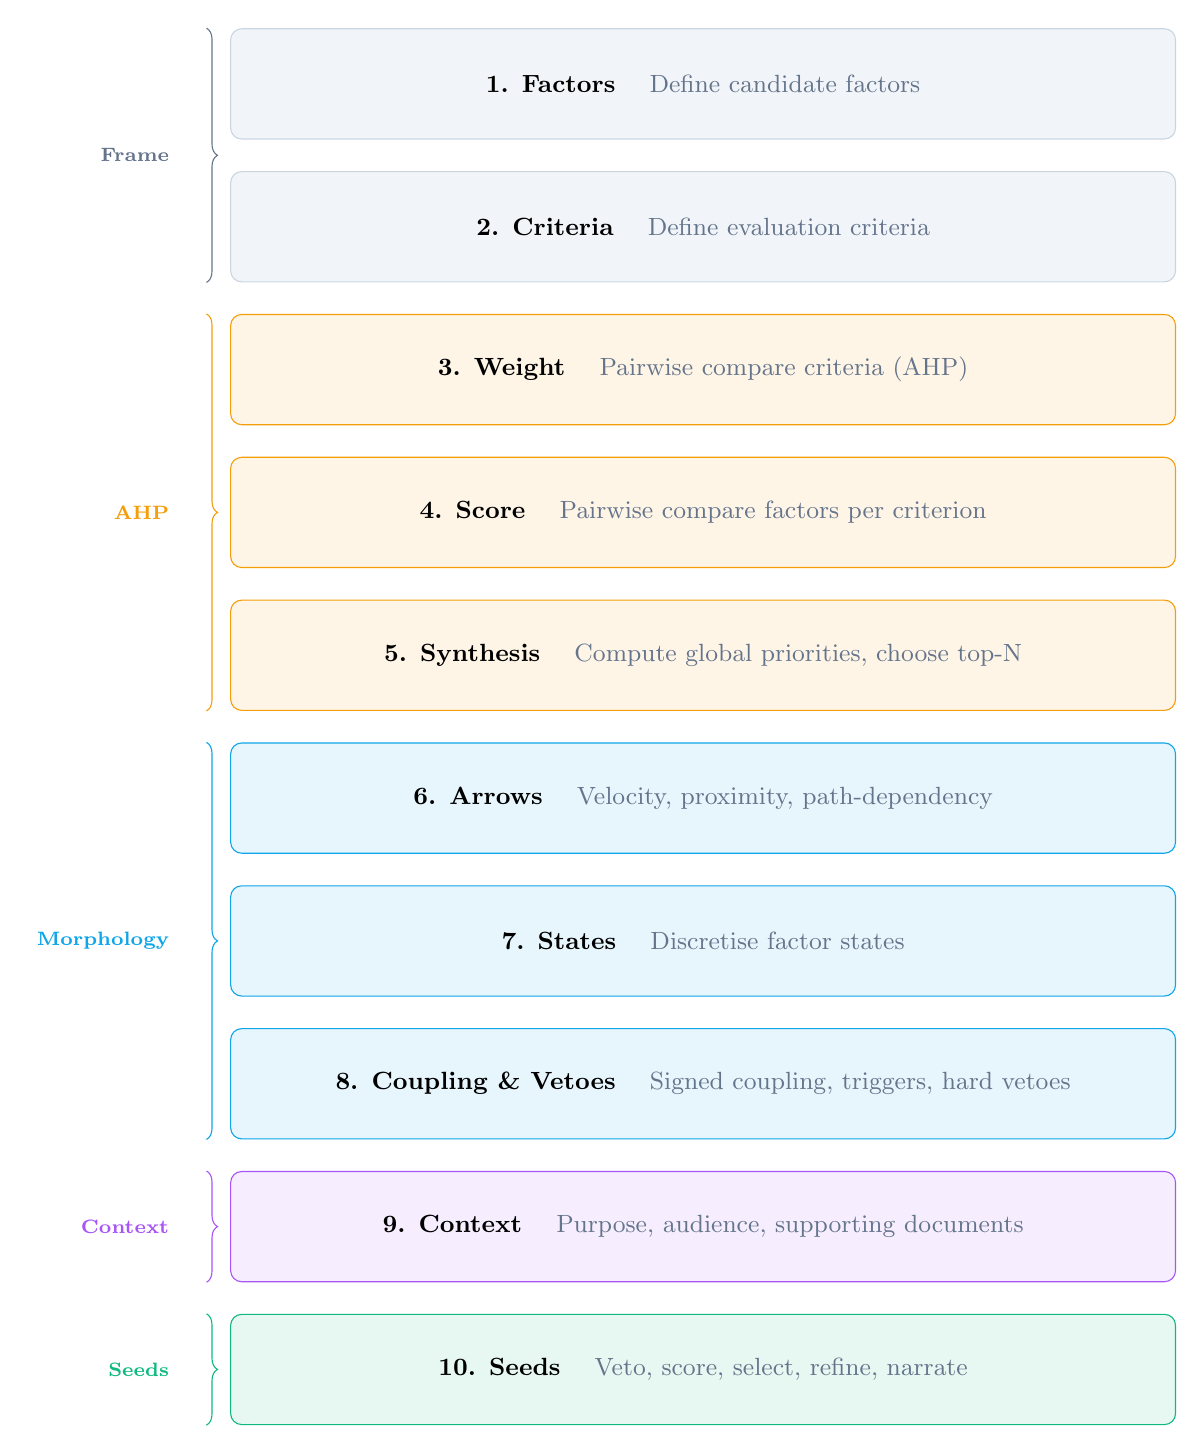
\begin{tikzpicture}[node distance=0.4cm, every node/.style={font=\scriptsize}]
  \node[layer, fill=slate100, draw=slate300] (s1) {\textbf{1. Factors} \quad{\color{slate500}Define candidate factors}};
  \node[layer, fill=slate100, draw=slate300, below=of s1] (s2) {\textbf{2. Criteria} \quad{\color{slate500}Define evaluation criteria}};
  \node[layer, fill=amber500!10, draw=amber500, below=of s2] (s3) {\textbf{3. Weight} \quad{\color{slate500}Pairwise compare criteria (AHP)}};
  \node[layer, fill=amber500!10, draw=amber500, below=of s3] (s4) {\textbf{4. Score} \quad{\color{slate500}Pairwise compare factors per criterion}};
  \node[layer, fill=amber500!10, draw=amber500, below=of s4] (s5) {\textbf{5. Synthesis} \quad{\color{slate500}Compute global priorities, choose top-N}};
  \node[layer, fill=sky500!10, draw=sky500, below=of s5] (s6) {\textbf{6. Arrows} \quad{\color{slate500}Velocity, proximity, path-dependency}};
  \node[layer, fill=sky500!10, draw=sky500, below=of s6] (s7) {\textbf{7. States} \quad{\color{slate500}Discretise factor states}};
  \node[layer, fill=sky500!10, draw=sky500, below=of s7] (s8) {\textbf{8. Coupling \& Vetoes} \quad{\color{slate500}Signed coupling, triggers, hard vetoes}};
  \node[layer, fill=violet500!10, draw=violet500, below=of s8] (s9) {\textbf{9. Context} \quad{\color{slate500}Purpose, audience, supporting documents}};
  \node[layer, fill=emerald500!10, draw=emerald500, below=of s9] (s10) {\textbf{10. Seeds} \quad{\color{slate500}Veto, score, select, refine, narrate}};

  \draw[decorate, decoration={brace, amplitude=4pt}, slate500] ($(s1.north west)+(-0.3,0)$) -- ($(s2.south west)+(-0.3,0)$) node[midway, left=10pt, font=\scriptsize\bfseries\color{slate600}, align=right] {Frame};
  \draw[decorate, decoration={brace, amplitude=4pt}, amber500] ($(s3.north west)+(-0.3,0)$) -- ($(s5.south west)+(-0.3,0)$) node[midway, left=10pt, font=\scriptsize\bfseries\color{amber500}, align=right] {AHP};
  \draw[decorate, decoration={brace, amplitude=4pt}, sky500] ($(s6.north west)+(-0.3,0)$) -- ($(s8.south west)+(-0.3,0)$) node[midway, left=10pt, font=\scriptsize\bfseries\color{sky500}, align=right] {Morphology};
  \draw[decorate, decoration={brace, amplitude=4pt}, violet500] ($(s9.north west)+(-0.3,0)$) -- ($(s9.south west)+(-0.3,0)$) node[midway, left=10pt, font=\scriptsize\bfseries\color{violet500}, align=right] {Context};
  \draw[decorate, decoration={brace, amplitude=4pt}, emerald500] ($(s10.north west)+(-0.3,0)$) -- ($(s10.south west)+(-0.3,0)$) node[midway, left=10pt, font=\scriptsize\bfseries\color{emerald500}, align=right] {Seeds};
\end{tikzpicture}
\caption{The ten-step pipeline grouped into five phases. AHP-related steps (3--5) produce factor weights with consistency checks. Morphological steps (6--8) characterise factor dynamics, states, coupling, and hard vetoes. Context (9) frames the AI generation. Seeds (10) is where the morphological search, selection, refinement, and narrative generation happen.}
\end{figure}

\subsection{Phases 1--2: Frame}

The strategist defines candidate factors — the forces, drivers, and uncertainties shaping the future being studied — and evaluation criteria. Defaults follow the GBN-plus-independence convention: Impact Magnitude, Uncertainty, Decision Relevance, Time Horizon Fit, Causal Independence. The fifth criterion is the explicit version of what experienced scenario planners do in their heads, preferring factors that operate independently rather than as proxies for some deeper variable.

\subsection{Phases 3--5: AHP weighting}

Pairwise comparisons among criteria using Saaty's nine-point scale produce a priority vector. The Consistency Ratio measures internal contradiction in the strategist's judgements. The same process is then applied to factors within each criterion separately, and the global priority of each factor is the weighted sum of its priorities across criteria. The strategist chooses how many top-ranked factors to carry into the morphological stage.

\subsection{Phases 6--8: Morphological characterisation with vetoes}

The strategist provides three new properties for each carried-forward factor: \textbf{velocity} (how fast the factor is approaching), \textbf{proximity to threshold} (how close to a tipping point), and \textbf{path-dependency} (how much accumulated past the factor carries). These produce a per-factor \emph{criticality score}: $\text{criticality}_i = v_i \cdot p_i \cdot (0.5 + 0.5 \cdot d_i)$. Factors with high criticality are the bifurcation candidates.

States are then defined — typically Low/Mid/High at numeric values $-1, 0, +1$. Coupling is scored on a signed scale from $-9$ (tightly damping) through $0$ (independent) to $+9$ (tightly reinforcing), with optional directional triggering chains.

\textbf{Hard vetoes} are declared in the same step as coupling. A veto is a factor-state pair the strategist marks as logically impossible — e.g.\ ``Memory Supply at High AND ASML Production at Low'' cannot coexist regardless of context. Vetoes are applied as an absolute filter before any soft scoring, eliminating the compensation effect inherent in pure aggregate-coupling.

\subsection{Phase 9: Strategic context}

The strategist provides purpose (the decision the scenarios will inform), audience descriptor (investors, board, policy, academic, workshop, mixed, custom), and supporting documents (pasted text, or uploaded \texttt{.txt}/\texttt{.md}/\texttt{.pdf}/\texttt{.docx} files). Each document carries an inclusion flag so the strategist can switch between context bundles without losing them. This context is consumed by the AI generation step in Phase 10 to ground narratives in the strategist's actual situation rather than producing generic foresight commentary.

\subsection{Phase 10: Seed generation, selection, narration}

The morphological space is enumerated exhaustively when $K^N \le 200{,}000$. Hard vetoes filter the space first; surviving seeds are scored on importance, coherence, and convergence; seeds above the coherence threshold $\tau$ are eligible for selection. The selection algorithm uses greedy farthest-first traversal followed by a hill-climbing refinement pass to maximise the alpha-weighted blend of mean score and minimum pairwise distance. Each selected seed is annotated with a non-linear arrival window estimated from factor velocity, proximity, and path-dependency.

Optional AI generation produces a structured markdown narrative for each seed — name, tagline, two-paragraph world description, structural tension, observable signals, and strategic implications — using the strategist's purpose, audience, and included documents.

% ============================================================
% PART V — MATHEMATICAL SPECIFICATION
% ============================================================
\section{Mathematical specification}

This section is normative. All formulas are expressed precisely and must be implemented as specified.

\subsection{Pairwise comparison and priority derivation}

A pairwise comparison matrix $A$ of size $n \times n$ satisfies $A_{ij} = 1/A_{ji}$ and $A_{ii} = 1$. Values are drawn from $\{1/9, 1/8, \ldots, 1/2, 1, 2, \ldots, 8, 9\}$ representing Saaty's intensity scale. The priority vector $w$ is derived via geometric-mean approximation:

\begin{equation}
w_i = \frac{\left(\prod_j A_{ij}\right)^{1/n}}{\sum_k \left(\prod_j A_{kj}\right)^{1/n}}
\end{equation}

The Consistency Ratio is computed as:

\begin{equation}
\lambda_{\max} = \frac{1}{n} \sum_i \frac{\sum_j A_{ij} \cdot w_j}{w_i}, \quad \text{CI} = \frac{\lambda_{\max} - n}{n - 1}, \quad \text{CR} = \frac{\text{CI}}{\text{RI}_n}
\end{equation}

where $\text{RI}_n$ is Saaty's tabulated Random Index. Required values: RI$_3$ = 0.58, RI$_4$ = 0.90, RI$_5$ = 1.12, RI$_6$ = 1.24, RI$_7$ = 1.32, RI$_8$ = 1.41, RI$_9$ = 1.45, RI$_{10}$ = 1.49. CR $\le 0.10$ is acceptable; $0.10 < \text{CR} \le 0.15$ is borderline; $\text{CR} > 0.15$ requires the matrix to be revised.

\subsection{Global factor weights}

For factor $i$ evaluated against criteria with weights $c_j$ and per-criterion factor priorities $p_{j,i}$:

\begin{equation}
W_i = \sum_j c_j \cdot p_{j,i}
\end{equation}

The top-$N$ factors by $W$ are carried into the morphological stage. Re-normalised weights $w'_i = W_i / \sum_{k \in \text{top}} W_k$ are used for seed scoring.

\subsection{Factor criticality}

Each carried-forward factor $i$ has an arrows profile $(v_i, p_i, d_i, \kappa_i)$ where $v_i, p_i, d_i \in [0, 1]$ are velocity, proximity, and path-dependency, and $\kappa_i \in [-1, 1]$ is consequence asymmetry (preserved for narrative annotation, not used in scoring). Criticality is:

\begin{equation}
\text{criticality}_i = v_i \cdot p_i \cdot (0.5 + 0.5 \cdot d_i)
\end{equation}

\subsection{Hard-veto filter}

A veto $V_{ij}^{ab}$ asserts that factor $i$ in state $a$ cannot coexist with factor $j$ in state $b$. The strategist's veto set is $\mathcal{V} = \{V_{ij}^{ab}\}$. Seed $S$ is admissible if and only if:

\begin{equation}
\forall (i, j) : i < j, \quad \neg V_{ij}^{S_i, S_j} \in \mathcal{V}
\end{equation}

Inadmissible seeds are removed before any scoring is computed. The hard-veto layer is the first filter applied after morphological enumeration.

\subsection{Seed scoring}

For seed $S$ with state values $\{v_0, \ldots, v_{K-1}\}$, factor weights $w'$, criticalities $c$, and signed coupling matrix $M \in [-9, 9]^{N \times N}$:

\paragraph{Importance.} AHP-weighted state deviation from neutral:
\begin{equation}
\text{importance}(S) = \frac{\sum_i w'_i \cdot |v_{S_i}|}{\sum_i w'_i \cdot \max_k |v_k|}
\end{equation}

\paragraph{Coherence.} Penalty for coupling-state mismatches. Let $c_{ij} = M_{ij}/9$ and $\delta_{ij} = |v_{S_i} - v_{S_j}|/(\max v - \min v)$. The pair penalty is:
\begin{equation}
P_{ij} = \begin{cases}
c_{ij} \cdot \delta_{ij} & \text{if } c_{ij} > 0 \quad \text{(reinforcing — penalise divergence)}\\
(-c_{ij}) \cdot (1 - \delta_{ij}) & \text{if } c_{ij} < 0 \quad \text{(damping — penalise alignment)}\\
0 & \text{otherwise}
\end{cases}
\end{equation}

\begin{equation}
\text{coherence}(S) = \max\left(0, \; 1 - \frac{\sum_{i<j} P_{ij}}{\sum_{i<j} |c_{ij}|}\right)
\end{equation}

\paragraph{Convergence potential.} Criticality-weighted state deviation, amplified by co-deviation:
\begin{align}
\text{baseConv}(S) &= \frac{\sum_i \text{criticality}_i \cdot |v_{S_i}|}{\max_k |v_k| \cdot \sum_i \text{criticality}_i}\\
A(S) &= \#\{i : \text{criticality}_i > 0.35 \land |v_{S_i}|/\max_k |v_k| > 0.5\}\\
\text{convergence}(S) &= \min\left(1, \; \text{baseConv}(S) \cdot \big(1 + 0.12 \cdot \max(0, A(S) - 1)\big)\right)
\end{align}

\paragraph{Combined score.} With user-controlled convergence focus $\varphi \in [0, 1]$:
\begin{equation}
\text{score}(S, \varphi) = \big((1-\varphi) \cdot \text{importance}(S) + \varphi \cdot \text{convergence}(S)\big) \cdot \text{coherence}(S)
\end{equation}

\subsection{Seed distance}

\begin{equation}
\text{distance}(S_a, S_b) = \frac{1}{\sum_i w'_i} \sum_i w'_i \cdot \frac{|v_{S_{a,i}} - v_{S_{b,i}}|}{\max v - \min v}
\end{equation}

\subsection{Diverse seed selection — greedy phase}

Given filtered seeds (those admissible under vetoes and passing coherence threshold $\tau$), target count $K_{\text{select}}$, and diversity weight $\alpha \in [0, 1]$:

\begin{enumerate}[leftmargin=*]
  \item Sort filtered seeds by score descending.
  \item Initialise $\text{Selected} = \{S_1\}$ where $S_1$ is the highest-scoring seed.
  \item While $|\text{Selected}| < K_{\text{select}}$ and remaining is non-empty:
    \begin{itemize}
      \item For each candidate $S_c$, compute $d_{\min}(S_c) = \min_{S \in \text{Selected}} \text{distance}(S_c, S)$.
      \item Compute utility $U(S_c) = \alpha \cdot \text{score}(S_c) + (1 - \alpha) \cdot d_{\min}(S_c)$.
      \item Add the candidate with highest $U$ to Selected.
    \end{itemize}
\end{enumerate}

\subsection{Diverse seed selection — hill-climbing refinement}

After greedy completion, refine the K-set by local search. The refinement objective is the global utility:

\begin{equation}
U_g(S) = \alpha \cdot \overline{\text{score}}(S) + (1 - \alpha) \cdot \min_{a, b \in S, a \ne b} \text{distance}(S_a, S_b)
\end{equation}

where $\overline{\text{score}}(S)$ is the mean score across the selected set. The refinement loop:

\begin{enumerate}[leftmargin=*]
  \item For each slot $k \in \{1, \ldots, K_{\text{select}}\}$:
    \begin{itemize}
      \item For each candidate $S_c$ not currently selected, evaluate $U_g$ on the trial set obtained by replacing slot $k$ with $S_c$.
      \item If any swap strictly improves $U_g$, accept the best one. Otherwise leave slot $k$ unchanged.
    \end{itemize}
  \item Repeat the slot pass until no swap is accepted, capped at 8 passes.
\end{enumerate}

The refinement converges quickly (2--4 passes for typical $K$) and corrects the myopic commitments of the greedy phase. Final per-seed annotation includes the average distance to the other selected seeds.

\subsection{Non-linear arrival window estimation}

For each carried-forward factor $i$ in seed $S$ whose state has $|v_{S_i}|/\max_k |v_k| \ge 0.4$, the arrival year is computed via a saturating sigmoid keyed on the full criticality product:

\begin{equation}
\text{years}_i = H \cdot \frac{1}{1 + \exp\big(\beta \cdot (\text{criticality}_i - 0.5)\big)}
\end{equation}

where $H$ is the planning horizon (default 15 years) and $\beta = 8$ is the sharpness parameter. The seed's arrival window is $(\min_i \text{years}_i, \; \text{median}_i \text{years}_i, \; \max_i \text{years}_i)$ over the qualifying factors.

\begin{figure}[H]
\centering
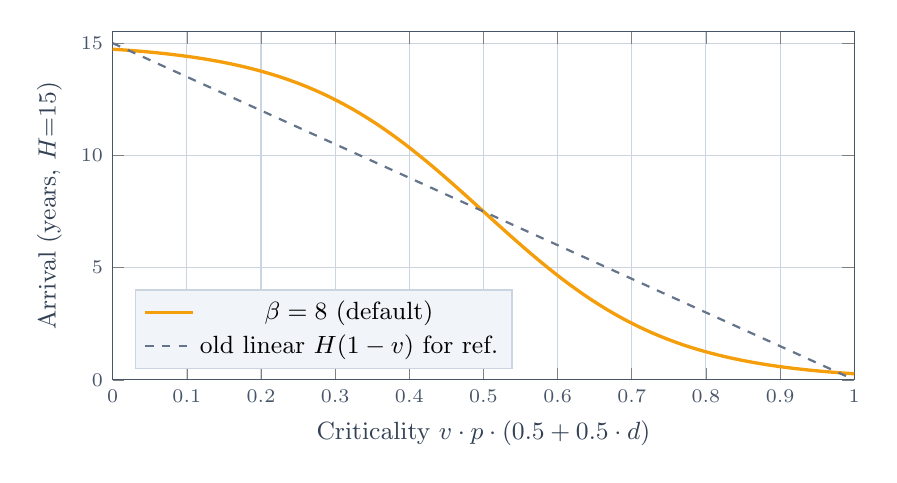
\begin{tikzpicture}
  \begin{axis}[
    width=11cm, height=6cm,
    xlabel={Criticality $v \cdot p \cdot (0.5 + 0.5 \cdot d)$},
    ylabel={Arrival (years, $H{=}15$)},
    xmin=0, xmax=1,
    ymin=0, ymax=15.5,
    grid=both,
    grid style={slate200},
    major grid style={slate300},
    axis line style={slate600},
    tick label style={font=\scriptsize, color=slate600},
    label style={font=\small, color=slate700},
    legend style={font=\scriptsize, draw=slate300, fill=slate100},
    legend pos=south west,
  ]
    \addplot[domain=0:1, samples=100, color=amber500, very thick] {15 / (1 + exp(8 * (x - 0.5)))};
    \addlegendentry{$\beta = 8$ (default)}
    \addplot[domain=0:1, samples=100, color=slate500, thick, dashed] {15 - 15*x};
    \addlegendentry{old linear $H(1 - v)$ for ref.}
  \end{axis}
\end{tikzpicture}
\caption{The non-linear arrival curve. Low-criticality factors arrive near the horizon; the steep transition through the middle captures the latent-then-cascade dynamic of complex adaptive systems; high-criticality factors with reinforcing coupling cluster their arrivals tightly near the present. Arrival timing is when a factor's force begins to bear on outcomes, not when a bifurcation ``happens'' — bifurcations emerge from the interaction of forces with different arrival patterns.}
\end{figure}

% ============================================================
% PART VI — ALGORITHMS AND MOTIVATIONS
% ============================================================
\section{Algorithms, motivations, and alternatives considered}

This section makes the design choices explicit. For each algorithmic component, it states the motivation, the chosen approach, and the principal alternatives that were considered and rejected, with reasons. Without this section, the methodology can be replicated but not understood; with it, the engineering team can defend or refine the choices on principled grounds.

\subsection{Algorithm A1 — AHP with geometric-mean priority derivation}

\textbf{Motivation.} The methodology requires defensible factor weights that can be audited by stakeholders. Pure intuition produces weights nobody can defend; rigid quantification produces weights nobody can populate. AHP threads the needle: it elicits judgement in the form humans are best at (pairwise comparisons), then derives a global priority vector with a built-in consistency check.

\textbf{Chosen approach.} Geometric-mean approximation of the principal eigenvector, with the standard Saaty 1--9 ratio scale and Consistency Ratio threshold of 0.10. CR is computed against Saaty's tabulated Random Indices.

\textbf{Alternatives considered.}

\begin{itemize}[leftmargin=*]
  \item \emph{Power-iteration eigenvector.} The mathematically pure form of priority derivation. Rejected because the geometric-mean approximation is faster, simpler to implement, and produces priorities that differ from the eigenvector solution by less than 1\% on typical reciprocal matrices. The implementation gain is real; the precision loss is invisible.
  \item \emph{Fuzzy AHP.} Replaces crisp Saaty intensities with triangular fuzzy numbers, producing range-based priority vectors that respect cognitive bounds under uncertainty. Considered seriously and rejected for v2.0 because it triples the elicitation burden (each comparison becomes three values: lower, central, upper), introduces interpretation complexity for non-technical audiences, and produces output ranges that the morphological pipeline does not currently consume. Recorded as a future-direction enhancement: the right shape is an opt-in advanced mode that surfaces priority bounds and runs a stress-test re-pipeline against them.
  \item \emph{Simos--Roy revised method.} Rank-and-weight elicitation using ordered cards and a single ratio judgement. Simpler than AHP but loses the per-pair auditability that makes AHP defensible to sceptical stakeholders. Rejected because the audit transparency is core to the tool's purpose.
  \item \emph{Direct weight elicitation.} Strategist types in numerical weights directly. Fastest possible but offers no consistency check and no audit trail. Rejected for the same reason.
\end{itemize}

\subsection{Algorithm A2 — Morphological enumeration with cap}

\textbf{Motivation.} The morphological space must be searchable in real time on a laptop. Brute-force enumeration is desirable when feasible because it eliminates algorithmic uncertainty about whether the global optimum has been found.

\textbf{Chosen approach.} Exhaustive enumeration of all $K^N$ seeds when this number is at most 200{,}000. Above the cap, the system shows an error and asks the strategist to reduce factors or states. Brute force at the default eight-factor three-state configuration produces 6{,}561 seeds, scored in under 100 ms.

\textbf{Alternatives considered.}

\begin{itemize}[leftmargin=*]
  \item \emph{NSGA-II evolutionary search.} Standard heuristic for multi-objective combinatorial optimisation. Considered as a fallback for spaces above the cap. Implementation deferred because the realistic operating range (eight to ten factors with three or five states) sits well within the brute-force regime; investing in NSGA-II would be premature optimisation.
  \item \emph{Simulated annealing.} Same reason for deferral as NSGA-II. Future direction if users routinely operate at the upper end of the morphological space.
  \item \emph{Sampling-based search.} Random sampling of $K^N$ space without exhaustive enumeration. Rejected because the loss of completeness guarantee is unacceptable for a tool intended to defend its selections to stakeholders.
\end{itemize}

\subsection{Algorithm A3 — Hard-veto filter}

\textbf{Motivation.} Aggregate-coupling alone has a known failure mode known as the \emph{compensation effect}: a fatal contradiction between two heavily coupled high-criticality factors can be mathematically masked by alignment elsewhere in the seed, producing a high coherence score that disguises a logically impossible configuration. This violates the foundational requirement that scenario seeds represent worlds that could actually exist.

\textbf{Chosen approach.} A two-layer filter. The first layer is a set of hard vetoes — explicit factor-state pairs the strategist marks as logically impossible. Vetoed seeds are filtered before any scoring is computed. The second layer is the soft aggregate-coupling coherence score, which captures graded incompatibility for everything not vetoed.

The two-layer structure recovers most of the rigour of full Cross-Consistency Assessment at a fraction of the elicitation cost. CCA in its strict form requires the strategist to mark every factor-state pair as compatible, marginal, or impossible — a load that scales as $\binom{N}{2} \cdot K^2$, rapidly impractical. Hard vetoes ask only for the genuinely impossible pairs, which the strategist can typically enumerate in a handful of declarations.

\textbf{Alternatives considered.}

\begin{itemize}[leftmargin=*]
  \item \emph{Full Cross-Consistency Assessment (Zwicky/Ritchey).} The orthodox form. Considered and rejected because the elicitation burden grows as $O(N^2 K^2)$ and reaches impractical density for the eight-factor three-state default (84 cells of pairwise judgement). The methodology becomes inaccessible to non-specialist strategists.
  \item \emph{Cross-Impact Balance Analysis (Weimer-Jehle).} Identifies internally consistent configurations as self-stabilising network equilibria, conceptually akin to Nash equilibria. Mathematically the most rigorous approach to scenario coherence. Rejected for v2.0 because populating the cross-impact matrix requires per-state-pair judgement at the same density as full CCA, plus equilibrium computation that is opaque to the strategist. The compensation-effect benefit captured is real but the implementation cost and elicitation burden are disproportionate to the marginal gain over hard-veto-plus-aggregate-coupling. Recorded as future direction for advanced workflows.
  \item \emph{Probabilistic coupling.} Treats each pairwise compatibility judgement as a Bayesian likelihood; coherence is the posterior probability of the seed configuration. Rejected because Knightian uncertainty makes the priors meaningless, and the posterior is therefore an artefact of the prior choice rather than a measurement of consistency.
\end{itemize}

\subsection{Algorithm A4 — Aggregate-coupling coherence}

\textbf{Motivation.} For configurations not caught by hard vetoes, the methodology still needs to surface the gradient of incompatibility. Two factors with strong reinforcing coupling don't generate impossibility when their states diverge — they generate tension that should reduce the seed's coherence score, all else equal.

\textbf{Chosen approach.} Signed coupling on a Saaty-style $-9$ to $+9$ scale, with a linear penalty function: reinforcing pairs penalise state divergence, damping pairs penalise state alignment. Coherence is normalised to $[0, 1]$ via division by the total possible absolute coupling.

\textbf{Alternatives considered.}

\begin{itemize}[leftmargin=*]
  \item \emph{Logical consistency rules.} Strategist writes propositional rules over factor states. Rejected because rule authoring is a software engineering task, not a strategic foresight task; the cognitive load shifts the methodology away from its target audience.
  \item \emph{Multiplicative coherence.} Coherence is the product of pairwise compatibility scores rather than $1 - \text{sum}$. Considered and rejected because multiplication amplifies single bad pairs into near-zero coherence even when the rest of the seed is internally consistent — too aggressive a punishment for soft incompatibilities. The hard-veto layer already handles cases where this aggressive punishment is warranted.
  \item \emph{Quadratic penalty.} Penalises divergent reinforcing pairs by the square of their state distance. Considered and rejected: the linear form is more interpretable and the squared form does not change the relative ordering of seeds enough to justify the loss of clarity.
\end{itemize}

\subsection{Algorithm A5 — Convergence potential with co-deviation amplifier}

\textbf{Motivation.} The methodology is interested in seeds where multiple high-criticality factors take extreme states simultaneously. This is not because forces ``arrive at the same time'' — the three arrows of time are continuous sources of force, always in play — but because such seeds represent regions of the morphological space where force interaction is structurally dense. When several high-criticality factors are simultaneously extreme, the coupling structure has more material to act on, and emergent third states (bifurcations in Arthur's sense) become structurally available. A seed where one critical factor is extreme and the others are neutral has thin interaction; a seed where three critical factors are simultaneously extreme has dense interaction. The scoring function must distinguish these cases. The metric is named \emph{convergence potential} for historical continuity but is more precisely characterised as \emph{interaction density}: how much potential the configuration has for coupled forces to combine into emergent outcomes.

\textbf{Chosen approach.} A criticality-weighted base measure of state extremity, amplified by a multiplicative factor that grows with the count of high-criticality factors at extreme states (the ``active count''). The amplifier is $1 + 0.12 \cdot \max(0, A(S) - 1)$, capping the convergence score at 1.

\textbf{Alternatives considered.}

\begin{itemize}[leftmargin=*]
  \item \emph{Pure base measure without amplifier.} Rejected because it fails to distinguish single-extreme-factor seeds from multi-extreme-factor seeds at similar criticality-weighted sums.
  \item \emph{Exponential amplifier.} Doubles convergence for each additional active factor. Rejected because it produces extreme rank inversions for small differences in active count, making the scoring brittle.
  \item \emph{Hard threshold.} Convergence is binary: 1 if active count $\ge 2$, 0 otherwise. Rejected because it loses the gradient information that lets the methodology rank seeds.
\end{itemize}

\subsection{Algorithm A6 — Diverse seed selection}

\textbf{Motivation.} The output set must span the morphological space rather than clustering around the local optimum of score. Stakeholders ask ``why these four scenarios rather than four others'' — the answer must be that the four are mutually distant under the weighted metric, not that they happen to be the top four by score.

\textbf{Chosen approach.} A two-phase algorithm. Phase one is greedy farthest-first traversal: pick the highest-scoring seed, then iteratively add the seed maximising the alpha-weighted blend of score and minimum distance to already-selected seeds. Phase two is hill-climbing refinement: for each slot in the selected set, try swapping with each non-selected candidate and accept any swap that improves the global utility (alpha-weighted blend of mean score and minimum pairwise distance).

The two-phase structure addresses a known failure mode of pure greedy farthest-first: the algorithm's myopia. Each greedy step considers only the relationship of the candidate to previously-selected seeds, not the structure of the final K-set. Greedy selections that look optimal at step three can turn out to be suboptimal once K is filled. The hill-climbing pass corrects these myopic commitments.

\textbf{Alternatives considered.}

\begin{itemize}[leftmargin=*]
  \item \emph{Pure greedy farthest-first.} The original v1.0 approach. Replaced because of the myopia failure mode, which manifests as outlier attraction (the algorithm reaches for fringe seeds that maximise local distance regardless of strategic relevance).
  \item \emph{$k$-Determinantal Point Processes.} Mathematically elegant — defines a probability distribution over all subsets of size $k$ that is proportional to the determinant of the kernel submatrix, encoding diversity as the volume of the spanned parallelepiped. Considered seriously and rejected for v2.0 because constructing the positive semi-definite kernel for morphological scenarios is non-trivial, exact MAP inference is NP-hard, and approximate algorithms add significant implementation complexity. The marginal quality gain over greedy-with-refinement is modest at the scale of $K=4$ from a few hundred filtered seeds. Recorded as future direction if the system scales to larger selection counts or larger candidate pools.
  \item \emph{Maximum sum diversification.} Selects the K-set maximising the sum of pairwise distances rather than the minimum. Rejected because it produces sets where two seeds can be very close as long as the others compensate — exactly the failure mode the methodology is trying to avoid.
  \item \emph{Genetic algorithms over K-sets.} Evolutionary search over candidate K-sets. Rejected for the same premature-optimisation reason as NSGA-II for individual seeds: at realistic problem scales, greedy-plus-refinement converges to the same answer faster and more transparently.
  \item \emph{Beam search.} Maintains a beam of partial K-set candidates rather than committing to the top one at each step. Considered and rejected because the beam complexity adds a tunable parameter (beam width) without producing meaningfully different results from greedy-plus-refinement at typical $K$.
\end{itemize}

\subsection{Algorithm A7 — Weighted Hamming distance}

\textbf{Motivation.} Distance between seeds must respect the AHP-derived weights — a difference on a heavyweight factor counts for more than the same difference on a lightweight factor. The metric must also be interpretable and computable in real time.

\textbf{Chosen approach.} Weighted Hamming distance: the AHP-weighted sum of normalised per-factor state differences, divided by the total weight to keep the metric in $[0, 1]$.

\textbf{Alternatives considered.}

\begin{itemize}[leftmargin=*]
  \item \emph{Unweighted Hamming distance.} Rejected because it ignores the strategist's prioritisation. Seeds differing on three lightweight factors and zero heavyweight factors would score equal to seeds differing on three heavyweight factors.
  \item \emph{Gower's distance.} Designed for mixed-type data; normalises per-variable differences by the variable's range. For uniformly ordinal factor states, Gower's reduces to weighted Hamming; the additional generality is unused. Considered and recorded as the right answer if the methodology ever supports continuous or binary factors alongside ordinal ones.
  \item \emph{Mahalanobis distance.} Accounts for inter-factor covariance. Rejected because the morphological space's covariance structure comes from the coupling matrix, which is already captured in the coherence score. Adding it to the distance metric would double-count.
  \item \emph{Structural Hamming Distance / Structural Intervention Distance.} Measures distance via the directed causal graph implied by triggering chains. Considered and rejected because it requires a richer causal graph than the coupling matrix represents, and because the chicken-and-egg problem of using a causal graph to compute distance between scenarios that are themselves outputs of the causal graph methodology is unresolved.
\end{itemize}

\subsection{Algorithm A8 — Non-linear arrival window}

\textbf{Motivation.} The original linear arrival formula, $\text{years}_i = (1 - v_i) \cdot H$, contradicts the complexity-economics intuition that underpins the methodology. Variables in turbulent fields do not progress smoothly toward a horizon at constant velocity; they accumulate latent tension and cascade rapidly past thresholds. A linear arrival model produces overconfident temporal predictions that mislead strategists about the suddenness of structural change.

\textbf{Chosen approach.} A saturating sigmoid arrival model keyed on the full criticality product $v_i \cdot p_i \cdot (0.5 + 0.5 \cdot d_i)$ rather than velocity alone. The sigmoid is centred at criticality 0.5 with sharpness $\beta = 8$. Low-criticality factors arrive near the horizon; high-criticality factors cluster near now; the steep transition through the middle captures the latent-then-cascade dynamic.

\textbf{Alternatives considered.}

\begin{itemize}[leftmargin=*]
  \item \emph{Markov chain transitions.} Translates the coupling matrix into a transition probability matrix; the arrival window is the expected number of steps for the chain to settle into an absorbing state. Mathematically elegant. Rejected for v2.0 because the strategist does not have data to populate honest transition probabilities; estimating them from the coupling matrix produces numbers that look like probabilities but are artefacts of the encoding.
  \item \emph{CIBSA (Cross-Impact Balance Simulated Annealing).} Adds a temperature parameter that simulates external systemic pressure, identifying metastable states. Rejected for the same reason: requires probability estimates the strategist cannot honestly produce.
  \item \emph{Power law $\text{years}_i = H \cdot (1 - v_i)^\gamma$.} Considered as a simpler non-linearity. Rejected because the curve is monotone in velocity but does not capture the path-dependency or proximity inputs, which the criticality-keyed sigmoid does.
  \item \emph{Discrete bucketed arrival (near, medium, far).} Avoids false precision by reporting only three categories. Considered and rejected because it removes the ability to compare arrival times across seeds, which the visualisation layer relies on.
\end{itemize}

\subsection{Algorithm A9 — AI scenario narrative generation}

\textbf{Motivation.} Selected seeds are starting positions for narrative work, and the writing of that narrative is itself substantial cognitive labour. AI generation can produce a credible first draft that the strategist refines, accelerating the path from seed to usable scenario.

\textbf{Chosen approach.} Each seed is rendered to a structured prompt containing the methodology framing, all factor states with weights and criticalities, all coupling and triggering relations, the arrival window, the seed's importance/coherence/convergence scores, and the strategist-provided strategic context (purpose, audience, included documents). The model is instructed to respond in markdown with a fixed section structure: \texttt{\#} title, italic tagline, \texttt{\#\# Narrative}, \texttt{\#\# Structural tension}, \texttt{\#\# Observable signals} (bulleted), \texttt{\#\# Strategic implications}.

The output is parsed by extracting each markdown section and rendering it through a typed display. Inline bold and italic are preserved.

\textbf{Alternatives considered.}

\begin{itemize}[leftmargin=*]
  \item \emph{JSON output with strict schema.} The original v1.0 approach. Replaced after observing systematic parsing failures from preamble text, markdown fences, smart quotes, trailing commas, and truncation mid-string. Markdown is the model's native output format for narrative content; forcing JSON degrades both writing quality and parsing reliability.
  \item \emph{Multi-turn refinement.} Generate, critique, refine across multiple model calls. Rejected for v2.0 because it triples API cost and latency for marginal narrative quality gain. Recorded as a future direction for high-stakes board-pack scenarios.
  \item \emph{Single bulk generation of all K seeds.} One prompt that generates four narratives together, with awareness of cross-seed contrast. Considered and rejected because the longer prompt and longer output substantially increase failure modes (truncation, attention dilution); the per-seed approach is more reliable and parallelisable. Recorded as a possible future enhancement when models reliably handle longer contexts.
  \item \emph{Templated narrative without LLM.} Pre-written narrative templates parameterised by factor states. Rejected because the resulting narratives are visibly mechanical and undermine the tool's credibility. The LLM provides the human-feeling specificity that templates cannot.
\end{itemize}

\subsection{Algorithm summary table}

\begin{table}[H]
\centering
\small
\begin{tabularx}{\textwidth}{@{}l X X@{}}
\toprule
\textbf{Component} & \textbf{Chosen} & \textbf{Headline alternative rejected} \\
\midrule
A1 Weighting        & Geometric-mean AHP             & Fuzzy AHP (elicitation cost) \\
A2 Enumeration      & Brute force, 200k cap          & NSGA-II (premature) \\
A3 Hard veto        & Explicit pair-veto set         & Full CCA (elicitation cost) \\
A4 Soft coherence   & Linear signed-coupling penalty & Multiplicative coherence (too aggressive) \\
A5 Convergence      & Linear amplifier on active count & Exponential amplifier (brittle) \\
A6 Selection        & Greedy + hill-climb refine     & $k$-DPP (implementation cost) \\
A7 Distance         & Weighted Hamming               & Structural Hamming (chicken-and-egg) \\
A8 Arrival          & Saturating sigmoid             & Markov chain (no honest priors) \\
A9 Narrative        & Markdown with structured sections & JSON schema (parsing fragility) \\
\bottomrule
\end{tabularx}
\caption{Summary of the algorithmic choices in v2.0 and the principal alternative considered and rejected for each. Detailed rationales appear in §6.}
\end{table}

% ============================================================
% PART VII — ARCHITECTURE
% ============================================================
\section{Software architecture}

The implementation follows hexagonal (ports and adapters) architecture as defined by Alistair Cockburn. The domain core has no knowledge of the outside world. All input/output flows through ports — TypeScript interfaces — implemented by adapters.

\begin{figure}[H]
\centering
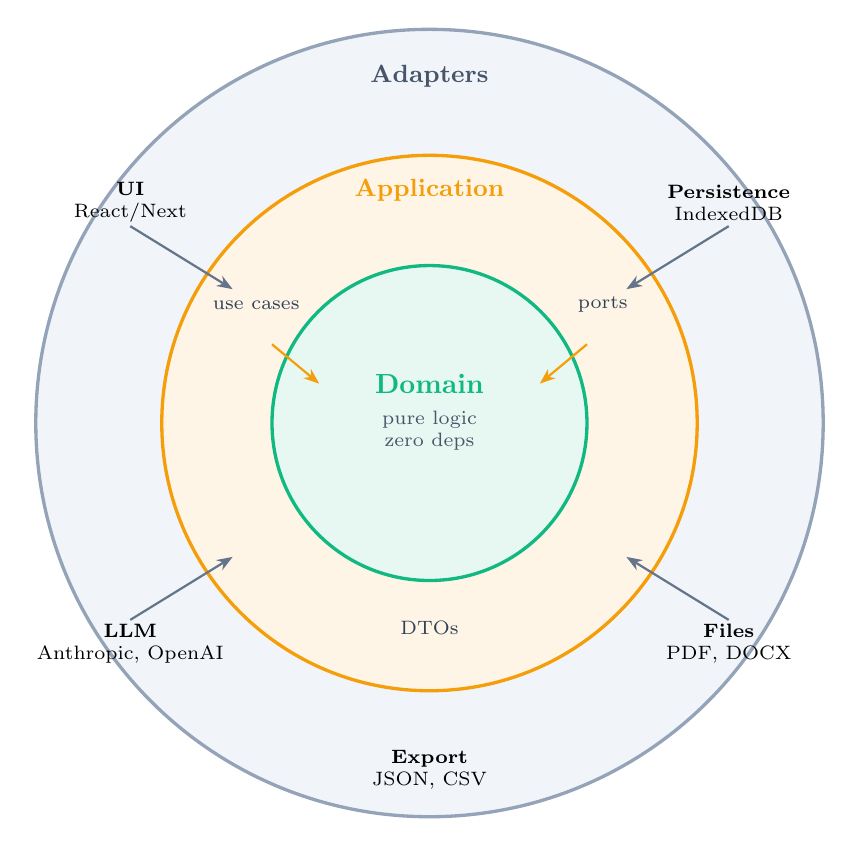
\begin{tikzpicture}[scale=1.0]
  \draw[draw=slate400, fill=slate100, very thick] (0,0) circle (5cm);
  \node[font=\small\bfseries\color{slate600}] at (0,4.4) {Adapters};
  \draw[draw=amber500, fill=amber500!10, very thick] (0,0) circle (3.4cm);
  \node[font=\small\bfseries\color{amber500}] at (0,2.95) {Application};
  \draw[draw=emerald500, fill=emerald500!10, very thick] (0,0) circle (2cm);
  \node[font=\bfseries\color{emerald500}] at (0,0.5) {Domain};
  \node[font=\scriptsize\color{slate600}, align=center] at (0,-0.1) {pure logic\\zero deps};
  \node[align=center, font=\scriptsize] at (-3.8,2.8) {\textbf{UI}\\React/Next};
  \node[align=center, font=\scriptsize] at (3.8,2.8) {\textbf{Persistence}\\IndexedDB};
  \node[align=center, font=\scriptsize] at (-3.8,-2.8) {\textbf{LLM}\\Anthropic, OpenAI};
  \node[align=center, font=\scriptsize] at (3.8,-2.8) {\textbf{Files}\\PDF, DOCX};
  \node[align=center, font=\scriptsize] at (0,-4.4) {\textbf{Export}\\JSON, CSV};
  \node[font=\scriptsize, color=slate700, align=center] at (-2.2,1.5) {use cases};
  \node[font=\scriptsize, color=slate700, align=center] at (2.2,1.5) {ports};
  \node[font=\scriptsize, color=slate700, align=center] at (0,-2.6) {DTOs};
  \draw[-{Stealth[length=2mm,width=1.5mm]}, slate500, thick] (-3.8,2.5) -- (-2.5,1.7);
  \draw[-{Stealth[length=2mm,width=1.5mm]}, slate500, thick] (3.8,2.5) -- (2.5,1.7);
  \draw[-{Stealth[length=2mm,width=1.5mm]}, slate500, thick] (-3.8,-2.5) -- (-2.5,-1.7);
  \draw[-{Stealth[length=2mm,width=1.5mm]}, slate500, thick] (3.8,-2.5) -- (2.5,-1.7);
  \draw[-{Stealth[length=2mm,width=1.5mm]}, amber500, thick] (-2.0,1.0) -- (-1.4,0.5);
  \draw[-{Stealth[length=2mm,width=1.5mm]}, amber500, thick] (2.0,1.0) -- (1.4,0.5);
\end{tikzpicture}
\caption{Hexagonal architecture. Dependency arrows point inward — adapters depend on application, application depends on domain, domain depends on nothing. The domain holds the mathematics; the application orchestrates use cases through ports; the adapters provide concrete I/O implementations.}
\end{figure}

\subsection{Layer responsibilities}

\begin{tabularx}{\textwidth}{lX}
\toprule
\textbf{Layer} & \textbf{Responsibility} \\
\midrule
\textbf{Domain} & Pure logic. Entities (Project, Factor, Criterion, FactorState, ScenarioSeed, Veto), value objects (SaatyIntensity, PairwiseMatrix, ArrowProfile, CouplingMatrix, VetoSet, SeedScore), and domain services (AHPCalculator, VetoFilter, SeedScorer, GreedySelector, RefinementPass, ArrivalEstimator). No external dependencies. No framework code. \\[3pt]
\textbf{Application} & Use cases that orchestrate domain logic and call ports. One use case per workflow step (DefineFactors, WeightCriteria, DeclareVetoes, GenerateSeeds, GenerateNarratives, etc.). Defines inbound ports (ProjectFacade) and outbound ports (ProjectRepository, LLMAdapter, FileTextExtractor, ExportService). \\[3pt]
\textbf{Adapters} & Concrete implementations of outbound ports. \texttt{IndexedDBProjectRepository}, \texttt{AnthropicLLMAdapter}, \texttt{OpenAILLMAdapter}, \texttt{PdfTextExtractor}, \texttt{DocxTextExtractor}, \texttt{JSONExportService}, \texttt{MarkdownScenarioParser}. Each adapter is replaceable without touching domain or application. \\[3pt]
\textbf{UI} & React/Next.js components. Server Components for static shell, Client Components for interactive content. Communicates only with the application layer through inbound ports — never imports domain types directly except as DTOs. \\
\bottomrule
\end{tabularx}

\subsection{Dependency rules}

Inner layers must not depend on outer layers. Specifically: domain depends on nothing; application depends only on domain; adapters depend on application and domain; UI depends on application (and may import shared types from the application layer). Enforce these rules through TypeScript path aliases and ESLint's \texttt{eslint-plugin-boundaries} rule, breaking the build on violations.

\subsection{Error handling}

The codebase uses a \texttt{Result<T, E>} discriminated union rather than throwing exceptions for expected failure modes (validation errors, inconsistent matrices, oversized seed spaces, malformed LLM responses). Unexpected errors may throw but must be caught at adapter boundaries and converted to \texttt{Result.err} before crossing into the application layer.

% ============================================================
% PART VIII — UI SPECIFICATION
% ============================================================
\section{User interface specification}

The UI implements a ten-step wizard. Each step is a self-contained component receiving project state via a hook (\texttt{useProject}) and dispatching through the inbound facade. Visual design uses a dark theme with the slate/amber palette; typography uses Fraunces (display), IBM Plex Sans (body), and JetBrains Mono (numerical).

\subsection{Visual design tokens}

\begin{tabularx}{\textwidth}{lX}
\toprule
\textbf{Token} & \textbf{Use} \\
\midrule
slate-950, slate-900 & background, surfaces \\
slate-800, slate-700 & borders, dividers \\
slate-300, slate-100 & primary and secondary text \\
amber-500, amber-400 & primary accent, active state, key controls \\
emerald-500, emerald-400 & reinforcing coupling, positive convergence \\
rose-500, rose-400 & damping coupling, vetoes, bifurcation flags \\
sky-500 & informational, links \\
violet-500 & strategic context indicators \\
\bottomrule
\end{tabularx}

\subsection{Step 8 — coupling and vetoes panel}

The coupling step combines three controls in one screen: signed coupling magnitude per pair, triggering chain direction per ordered pair, and hard-veto declarations. The veto declarator is a separate sub-panel below the coupling matrix, with two factor pickers, two state pickers, an ``$\otimes$ cannot coexist with'' indicator, and an Add button. Declared vetoes appear as removable rows with the factor names, the impossible states in rose pills, and an X for removal.

\subsection{Step 10 — seed selection and narrative generation}

The seeds step renders the selected K-set as cards, each containing the seed's name (editable), bifurcation phase tag (pre/mid/post/steady), four metric badges (importance, coherence, convergence, distance), the arrival window with arriving-factor list, the factor-state grid coloured by criticality, and an AI generation panel.

The AI generation panel has three states: empty (with a ``Generate with AI'' button), generating (with a spinner), and rendered (with the markdown narrative split into structured sections plus a regenerate link).

The stats grid above the cards shows seed-space size, vetoed-out count (when vetoes are active), seeds above coherence threshold, filter rate, and selected count. A context-active badge confirms the AI generation will use the strategist-supplied purpose and documents.

\subsection{Output visualisations}

Two principal visualisations communicate the seed set:

\textbf{Parallel coordinates plot.} Each selected seed is rendered as a polyline through factor-state space. Axes are coloured by criticality — red for high (above 0.5), amber for moderate (0.3--0.5), slate for low. Mathematical distinctiveness is immediately visible: if the polylines diverge significantly across the parallel axes, the seeds genuinely span different futures; if they cluster, the diversity parameter or factor weights need re-examination.

\textbf{Arrival timeline.} All seeds plotted on a 0-to-15-year horizon with median markers and range bars showing the arrival window from the saturating sigmoid model. The temporal spread of the seed set is immediately legible — which scenarios arrive soon versus which remain distant.

% ============================================================
% PART IX — DEPLOYMENT
% ============================================================
\section{Deployment}

The tool deploys as a single-page web application. Two deployment paths are supported, reflecting different stages of validation maturity.

\subsection{V1 path — minimal Next.js wrapper}

Suitable when the methodology is still being validated against real strategic problems. The existing JSX prototype is dropped into a Next.js App Router project as a single Client Component, with one functional change: an API key input is added to capture the user's Anthropic credentials, persisted in localStorage. No architectural refactor. Deployment to Vercel via \texttt{vercel --prod}.

This path optimises for time-to-validation. Architectural rigour is deferred until the methodology has earned its keep on real decisions.

\subsection{V2 path — hexagonal Next.js refactor}

Suitable once v1 has produced enough validated decisions to justify the engineering investment. The methodology is extracted into a framework-agnostic domain layer; use cases live in an application layer; React/Next.js becomes the UI adapter. Outbound ports and adapters cover persistence (IndexedDB), LLM (Anthropic and OpenAI), file extraction (PDF.js and Mammoth.js, lazy-loaded), and export (JSON, CSV).

ESLint with \texttt{eslint-plugin-boundaries} enforces layer dependency rules at build time. Test coverage targets are 95\% for domain, 80\% for application, 60\% for UI. Property-based tests via fast-check cover priority-vector invariants, coherence bounds, and selection-set distance properties.

\subsection{Privacy posture}

Both paths use a bring-your-own-key model. The user's API key is stored in browser-local storage (localStorage in v1, IndexedDB in v2), never transmitted to any server other than the chosen LLM provider. No backend, no proxy, no telemetry. Documents uploaded for AI context are processed entirely client-side; only the text the user explicitly chooses to include in generation reaches the LLM provider.

This posture is documented prominently in the README and is non-negotiable. Any future feature that would require server-side key handling — for instance, billing-managed access for non-technical users — must use a separate adapter and a clearly distinct deployment.

% ============================================================
% PART X — IMPLEMENTATION PHASING
% ============================================================
\section{Implementation phasing}

The v2 work decomposes into nine phases, each independently shippable.

\begin{enumerate}[leftmargin=*]
  \item \textbf{Domain core.} Value objects, domain services, AHP calculator. Full unit and property-based test coverage. No UI.
  \item \textbf{Morphological core.} Arrows, coupling, veto filter, space generator, scorer, greedy selector, hill-climb refinement, sigmoid arrival estimator. Snapshot regression on default fixture.
  \item \textbf{Application layer.} Project aggregate, all use cases, in-memory repository.
  \item \textbf{UI scaffolding.} Next.js shell, routing, theme, layout, step navigation.
  \item \textbf{UI steps 1--5.} AHP-related steps. End-to-end happy path through synthesis.
  \item \textbf{UI steps 6--8.} Arrows, states, coupling-and-vetoes. Default fixture produces correct output through Step 8.
  \item \textbf{UI steps 9--10.} Strategic context, seeds, parallel coordinates, arrival timeline. AI generation in markdown with structured rendering.
  \item \textbf{Persistence and LLM adapters.} IndexedDB, Anthropic and OpenAI adapters with API-key settings panel, file extractors.
  \item \textbf{Export adapters and deployment.} JSON/CSV export, README, Vercel/Cloudflare/Netlify configs, Lighthouse pass.
\end{enumerate}

\subsection{Acceptance criteria}

The system is considered complete when the following are demonstrably true:

\begin{itemize}[leftmargin=*]
  \item A user can complete the ten-step wizard end-to-end using the default fixture and produce four named, phase-tagged scenario seeds.
  \item All consistency ratios above 15\% are visibly flagged with guidance on resolution.
  \item Hard vetoes filter the morphological space before scoring; the vetoed-out count is surfaced when any veto is active.
  \item The hill-climbing refinement strictly improves global utility relative to greedy-only selection on at least one of three benchmark fixtures.
  \item The seed set for the default fixture matches a committed snapshot to within $10^{-9}$ numerical tolerance on all scores.
  \item AI generation works with a user-supplied API key for both Anthropic and OpenAI providers, with markdown output reliably parsed.
  \item File uploads work for \texttt{.txt}, \texttt{.md}, \texttt{.pdf}, and \texttt{.docx}.
  \item Project state persists across page reloads via IndexedDB.
  \item Lighthouse accessibility score $\ge 95$ on the seeds page.
  \item Production bundle under 350 KB gzipped initial route, with PDF/DOCX extractors as separate lazy chunks.
\end{itemize}

% ============================================================
% PART XI — DEFAULT CONFIGURATION
% ============================================================
\section{Default configuration}

For reference and snapshot testing, the default fixture is:

\begin{tabularx}{\textwidth}{lX}
\toprule
\textbf{Element} & \textbf{Default value} \\
\midrule
Factors & AI Capability Progress Rate, RL Paradigm Replacement, ASML/EUV Tool Production, Memory Supply (HBM/DRAM), Lab AGI-Pilledness, China-West Divergence, US Power and Data Centre Scaling, AGI Economic Integration Mode \\
Criteria & Impact Magnitude, Uncertainty, Decision Relevance, Time Horizon Fit, Causal Independence \\
Top-N & 8 (all factors carried forward) \\
States & Low ($-1$), Mid ($0$), High ($+1$) \\
Default arrow & velocity 0.5, proximity 0.5, path-dep 0.5, consequence 0 (overridden per factor in fixture) \\
Default coupling & non-zero on transcript-derived pairs (see fixture file) \\
Default vetoes & none (strategist declares per project) \\
$K_{\text{select}}$ & 4 \\
$\alpha$ (diversity weight) & 0.5 \\
$\varphi$ (convergence focus) & 0.6 \\
$\tau$ (coherence threshold) & 0.4 \\
$\beta$ (arrival sharpness) & 8 \\
Horizon years $H$ & 15 \\
Seed-space cap & 200{,}000 \\
Refinement pass cap & 8 \\
LLM model & \texttt{claude-sonnet-4-5-20250929} (configurable) \\
LLM max tokens & 2000 \\
\bottomrule
\end{tabularx}

% ============================================================
% PART XII — GLOSSARY
% ============================================================
\section{Glossary}

\begin{description}[leftmargin=2.5cm, style=nextline]
  \item[AHP] Analytic Hierarchy Process. Saaty's method for deriving priority weights from pairwise comparisons.
  \item[Bifurcation] An emergent state produced when forces from different temporal origins (the three arrows) interact in ways neither force would have produced independently. Borrowed from chaos theory; central to Arthur's complexity economics. The methodology surfaces bifurcation candidates as seeds where coupled high-criticality factors take extreme values simultaneously, indicating dense force interaction in that region of the morphological space.
  \item[Coherence] Property of a scenario seed measuring internal consistency under coupling constraints. High when reinforcing-coupled factors share state direction and damping-coupled factors oppose. The aggregate-coupling soft layer of the two-layer filter.
  \item[Compensation effect] Failure mode of pure aggregate-coupling: a fatal contradiction between two heavily coupled factors masked by alignment elsewhere in the seed. Defeated in v2.0 by hard vetoes.
  \item[Convergence Potential] Property of a scenario seed measuring \emph{interaction density} — the degree to which high-criticality factors are simultaneously at extreme states, creating the structural conditions for forces from different temporal origins to interact. The name is historical; the concept is best understood as how much material the coupling structure has to work with in this configuration. Not to be confused with temporal convergence; the three arrows of time are forces in continuous play, not events that meet at a moment.
  \item[Criticality] Per-factor property derived from velocity $\times$ proximity, amplified by path-dependency. Identifies factors most likely to drive bifurcation.
  \item[GBN] Global Business Network, the consultancy where the intuitive-logics scenario method was codified by Schwartz, Wack, and Ogilvy in the 1980s.
  \item[Hard veto] Strategist-declared factor-state pair marked as logically impossible. Filters seeds before scoring.
  \item[Hill-climbing refinement] Local-search post-process applied to the greedy farthest-first K-set, swapping each slot against non-selected candidates to improve global utility.
  \item[Knightian Uncertainty] Frank Knight's distinction between calculable risk and irreducible uncertainty.
  \item[Morphological Analysis] Zwicky's method for systematically exploring multi-dimensional configuration spaces by enumerating combinations of factor states.
  \item[OSPA] Oxford Scenario Planning Approach. Saïd Business School's variant of intuitive-logics scenario planning, distinguished by the three arrows of time and the contextual/transactional environment split.
  \item[Saturating sigmoid arrival] Non-linear arrival window model keyed on the criticality product, replacing the v1.0 linear formula. Captures the latent-then-cascade dynamic of complex adaptive systems.
  \item[Seed] A vector of factor-state assignments representing a starting position for narrative scenario development. Not a finished scenario.
  \item[TUNA] Turbulent, Unpredictable, Novel, Ambiguous. Oxford's term for the conditions that justify scenario planning over forecasting.
\end{description}

% ============================================================
% REFERENCES
% ============================================================
\section*{Selected references}

\begin{itemize}[leftmargin=*]
  \item Arthur, W. B. (2009). \textit{The Nature of Technology: What It Is and How It Evolves}. Free Press.
  \item Cockburn, A. (2005). Hexagonal architecture. \textit{alistair.cockburn.us}.
  \item Emery, F. E., \& Trist, E. L. (1965). The causal texture of organizational environments. \textit{Human Relations}, 18(1), 21--32.
  \item Knight, F. H. (1921). \textit{Risk, Uncertainty, and Profit}. Houghton Mifflin.
  \item Kulesza, A., \& Taskar, B. (2012). Determinantal point processes for machine learning. \textit{Foundations and Trends in Machine Learning}, 5(2--3), 123--286.
  \item Ramírez, R., \& Wilkinson, A. (2016). \textit{Strategic Reframing: The Oxford Scenario Planning Approach}. Oxford University Press.
  \item Ritchey, T. (2011). \textit{Wicked Problems -- Social Messes: Decision Support Modelling with Morphological Analysis}. Springer.
  \item Saaty, T. L. (1977). A scaling method for priorities in hierarchical structures. \textit{Journal of Mathematical Psychology}, 15(3), 234--281.
  \item Schwartz, P. (1991). \textit{The Art of the Long View}. Doubleday.
  \item van der Heijden, K. (1996). \textit{Scenarios: The Art of Strategic Conversation}. Wiley.
  \item Weimer-Jehle, W. (2006). Cross-impact balances: A system-theoretical approach to cross-impact analysis. \textit{Technological Forecasting and Social Change}, 73(4), 334--361.
  \item Zwicky, F. (1969). \textit{Discovery, Invention, Research -- Through the Morphological Approach}. Macmillan.
\end{itemize}

\vfill
\hrule
\vspace{0.5em}
\noindent\textit{\small\color{slate500} End of document. Version 2.0 \textbullet{} Hard vetoes, hill-climb refinement, sigmoid arrival, AI generation, deployment specification.}

\end{document}
